\chapter{Le sang et l'appareil circulatoire}\label{ch:b2:blood-circulation}

En 1628, William Harvey fit un calcul. Le cœur, estimait-il, contient
environ deux onces de \omterm{def:b2:blood-circulation:blood}{sang} et bat soixante-dix fois par minute~; même si
une fraction seulement en était expulsée à chaque battement, le cœur
pomperait en une heure plusieurs fois le poids du corps entier. Le \omterm{def:b2:blood-circulation:blood}{sang}
ne pouvait pas être fabriqué et consommé à ce rythme, comme Galien
l'enseignait depuis quatorze siècles~: il devait tourner en rond. Puis
il le démontra~: serrez un lien autour du bras, et les \omterm{def:b2:blood-circulation:vessels}{veines} situées en
dessous du lien gonflent, non celles du dessus~; poussez le \omterm{def:b2:blood-circulation:blood}{sang} d'une
\omterm{def:b2:blood-circulation:vessels}{veine} vers la main, au-delà d'une valvule, et il refuse d'avancer. Le
\omterm{def:b2:blood-circulation:blood}{sang} est pompé dans les \omterm{def:b2:blood-circulation:vessels}{artères}, revient par les \omterm{def:b2:blood-circulation:vessels}{veines}, et les cinq
litres passent tout entiers par le cœur chaque minute. Ce chapitre
traite de ce système clos --- ce qu'est le \omterm{def:b2:blood-circulation:blood}{sang}, comment il est
acheminé, la physique de son écoulement dans les vaisseaux, de l'aorte
à un \omterm{def:b2:blood-circulation:vessels}{capillaire}, et les échanges, dans les \omterm{def:b2:blood-circulation:vessels}{capillaires}, qui sont la
raison d'être de l'ensemble.

\section{Le sang}

\begin{definition}[La composition du sang]\label{def:b2:blood-circulation:blood}
\index{sang}\index{plasma}\index{hematocrite@hématocrite}\index{hematie@hématie}\index{plaquette}
Le sang est un tissu en suspension~: environ \qty{5}{L} chez l'adulte,
\qty{7}{\%} de la masse corporelle. Centrifugé, il se sépare en
\emph{plasma} (\qty{55}{\%}~: de l'eau, \qty{70}{g/L} de protéines ---
albumine, globulines, fibrinogène --- et les sels, sucres, lipides, gaz
et hormones qu'il transporte) et en cellules (\qty{45}{\%}, c'est
l'\emph{hématocrite})~: les \emph{hématies} ($5\times 10^{12}$ par
litre, disques biconcaves de \qty{7}{\micro m} sans noyau, chacun rempli
de \num{280} millions de molécules d'hémoglobine, vivant 120 jours et
produits par la moelle osseuse à raison de deux millions par seconde),
les \emph{leucocytes} ($7\times 10^{9}$ par litre~: granulocytes
neutrophiles, lymphocytes, monocytes, granulocytes éosinophiles et
basophiles, le bras mobile de l'immunité) et les \emph{plaquettes}
($3\times 10^{11}$ par litre, fragments de cellules de la moelle qui
obturent les plaies et déclenchent la coagulation). Les hématies
transportent le dioxygène --- \qty{200}{mL} par litre de sang à
saturation complète, soixante-dix fois ce que dissout l'eau --- et le
plasma transporte tout le reste, y compris les \qty{20}{\%} du
$\mathrm{CO_2}$ qui ne sont pas dans les cellules, la chaleur des
muscles jusqu'à la peau, et les hormones du
\cref{ch:b2:cell-signalling} jusqu'à leurs cibles. Le sang est aussi
une solution soumise à une \emph{\omterm{thm:b2:blood-circulation:oncotic}{pression oncotique}}~: ses protéines,
qui ne peuvent pas quitter les \omterm{def:b2:blood-circulation:vessels}{capillaires}, exercent une attraction
osmotique d'environ \qty{25}{mmHg}, et c'est cette attraction qui
retient le plasma dans les vaisseaux.
\end{definition}

\begin{omfigure}
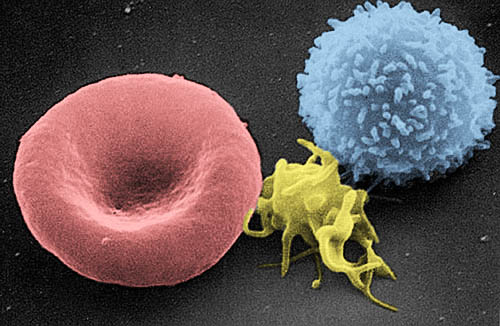
\includegraphics[width=0.5\linewidth]{images/book3/red-cells-nci.jpg}

{\small Une \omterm{def:b2:blood-circulation:blood}{hématie}, une \omterm{def:b2:blood-circulation:blood}{plaquette} et un leucocyte (un lymphocyte) au
microscope électronique à balayage~: les trois composants cellulaires du
\omterm{def:b2:blood-circulation:blood}{sang}, à la même échelle.}
\end{omfigure}

\begin{proposition}[L'hémostase]\label{prop:b2:blood-circulation:clotting}
\index{hemostase@hémostase}\index{cascade de la coagulation}\index{fibrine}
Un vaisseau sectionné est obturé en trois étapes, en quelques minutes.
Le vaisseau se contracte~; les \omterm{def:b2:blood-circulation:blood}{plaquettes} adhèrent au collagène mis à
nu, libèrent des signaux qui recrutent et activent d'autres \omterm{def:b2:blood-circulation:blood}{plaquettes},
et forment un clou~; et une \emph{cascade} de protéases plasmatiques,
chacune activant la suivante (une douzaine de facteurs de la
coagulation, pour la plupart produits par le foie, plusieurs exigeant
la vitamine K), convertit le fibrinogène en \emph{fibrine} insoluble,
dont les filaments enserrent le clou dans un caillot. Une cascade
amplifie~: une trace du déclencheur (le facteur tissulaire de la paroi
lésée) aboutit à des grammes de fibrine. Elle doit aussi être
contenue~: des anticoagulants du \omterm{def:b2:blood-circulation:blood}{plasma} (antithrombine, protéine C) et
de l'endothélium intact cantonnent le caillot à la plaie, et un second
système, la fibrinolyse, le dissout à mesure que le vaisseau cicatrise.
L'hémophilie est l'absence d'un facteur~; une thrombose est un caillot
là où il n'en fallait pas, et la première cause de mortalité dans les
pays riches est un caillot dans une \omterm{def:b2:blood-circulation:vessels}{artère} coronaire ou cérébrale.
\end{proposition}

\section{Les circuits}

\begin{definition}[Ouverte et fermée, simple et double]\label{def:b2:blood-circulation:circuits}
\index{circulation ouverte}\index{circulation fermee@circulation fermée}\index{double circulation}\index{circulation pulmonaire}\index{circulation systemique@circulation systémique}
Dans une circulation \emph{ouverte} (insectes, la plupart des
mollusques), un cœur pompe le \omterm{def:b2:blood-circulation:blood}{sang} dans une cavité du corps où il baigne
directement les organes et revient à basse pression~; l'écoulement est
lent et mal dirigé, et les insectes ont dissocié le problème des gaz de
celui du \omterm{def:b2:blood-circulation:blood}{sang} en conduisant l'air directement jusqu'aux tissus. Dans une
circulation \emph{fermée} (annélides, céphalopodes, vertébrés), le \omterm{def:b2:blood-circulation:blood}{sang}
reste dans des vaisseaux et est poussé sous pression à travers les
\omterm{def:b2:blood-circulation:vessels}{capillaires}, si bien que sa distribution peut être réglée organe par
organe. Les poissons ont une circulation \emph{simple}~: cœur
$\to$ branchies $\to$ corps $\to$ cœur, si bien que le \omterm{def:b2:blood-circulation:blood}{sang} atteint les
tissus à la faible pression qui subsiste après les \omterm{def:b2:blood-circulation:vessels}{capillaires}
branchiaux. Les mammifères et les oiseaux ont une circulation
\emph{double}~: le cœur droit assure la circulation \emph{pulmonaire}
(poumons, basse pression, \qty{25}{mmHg} en systole) et le cœur gauche,
après le retour du \omterm{def:b2:blood-circulation:blood}{sang}, la circulation \emph{systémique} (corps, haute
pression, \qty{120}{mmHg})~; les deux pompes sont en série et déplacent
le même débit, environ \qty{5}{L} par minute au repos. Les amphibiens et
la plupart des reptiles ont un cœur à ventricule unique qui mélange en
partie les deux courants --- le stade intermédiaire. La circulation
double est ce qui rend possible le métabolisme d'un endotherme~: une
haute pression pour chaque organe et un poumon protégé de cette
pression.
\end{definition}
\begin{proof}[Faits expérimentaux]
Harvey (1628) argumenta à partir de la quantité --- le débit calculé
ci-dessus --- et de la structure~: les valvules des \omterm{def:b2:blood-circulation:vessels}{veines}, décrites par
Fabricius, ne laissent passer le \omterm{def:b2:blood-circulation:blood}{sang} que vers le cœur, comme il le
montra en appuyant sur les \omterm{def:b2:blood-circulation:vessels}{veines} d'un bras ligaturé~; les valves du
cœur ne le laissent passer que des oreillettes aux ventricules puis aux
\omterm{def:b2:blood-circulation:vessels}{artères}~; et le \omterm{def:b2:blood-circulation:blood}{sang} jaillit des \omterm{def:b2:blood-circulation:vessels}{artères}, alors qu'il suinte des
\omterm{def:b2:blood-circulation:vessels}{veines}. Il ne pouvait pas voir les \omterm{def:b2:blood-circulation:vessels}{capillaires} et en déduisit
l'existence~; Malpighi les observa dans un poumon de grenouille en 1661,
quatre ans après la mort de Harvey.
\end{proof}

\begin{omfigure}
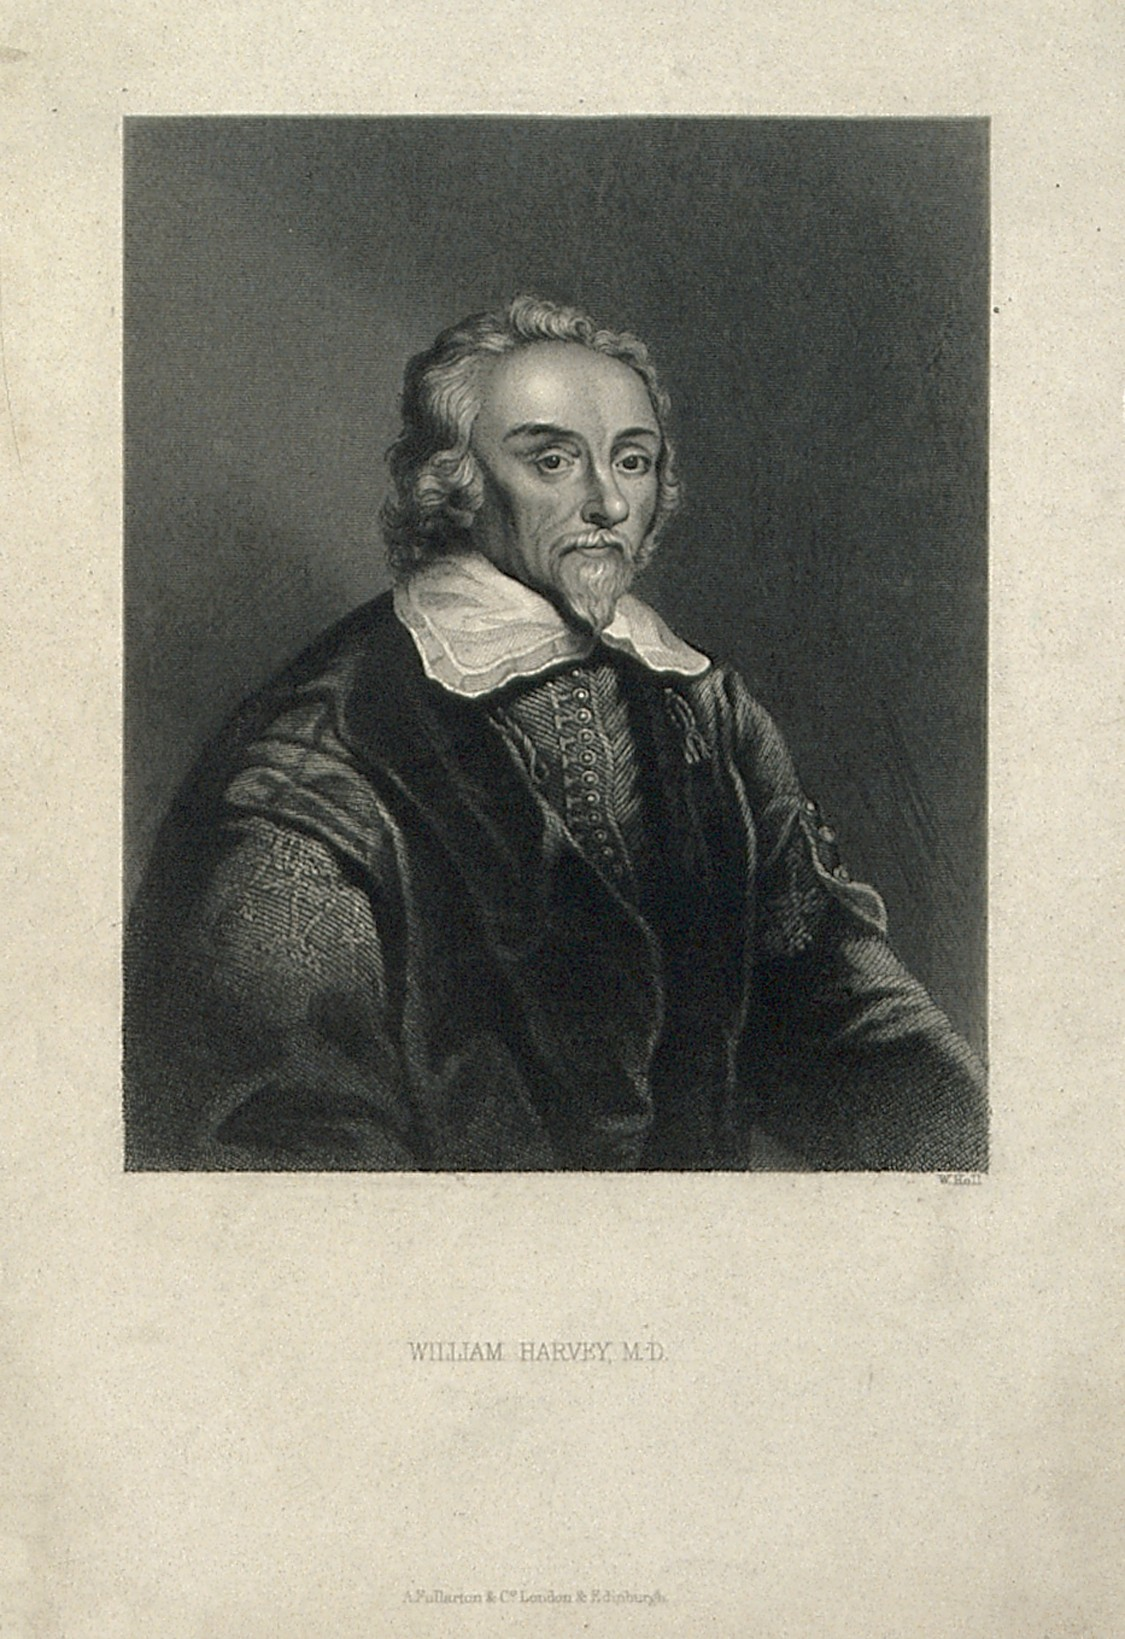
\includegraphics[width=0.3\linewidth]{images/book4/harvey.jpg}\hspace{0.05\linewidth}
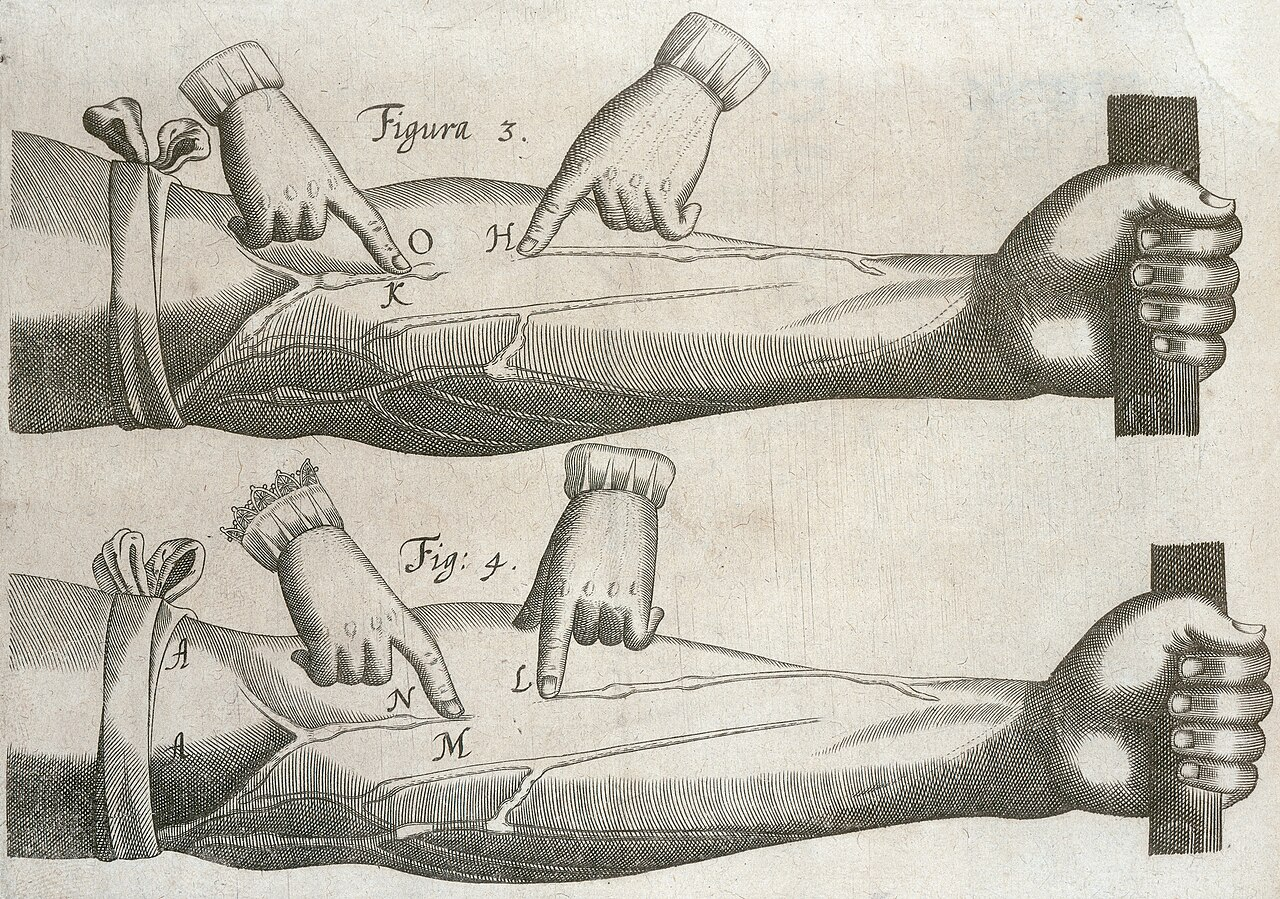
\includegraphics[width=0.42\linewidth]{images/book4/harvey-veins.jpg}

{\small William Harvey, et la planche de son livre de 1628~: les \omterm{def:b2:blood-circulation:vessels}{veines}
d'un avant-bras ligaturé gonflent en dessous du lien, et le \omterm{def:b2:blood-circulation:blood}{sang} poussé
vers la main s'arrête aux valvules.}
\end{omfigure}

\begin{omfigure}
\begin{tikzpicture}[every node/.style={font=\scriptsize}, >=stealth]
  % lungs and body
  \node[draw, rounded corners, fill=omDef!12, minimum width=3.4cm, minimum height=0.9cm] (lung) at (0,3) {poumons~: capillaires pulmonaires};
  \node[draw, rounded corners, fill=omExo!25, minimum width=3.4cm, minimum height=0.9cm] (body) at (0,-3) {corps~: capillaires systémiques};
  % heart chambers
  \node[draw, fill=omDef!25, minimum width=1.3cm, minimum height=0.7cm] (ra) at (-1.6,0.6) {oreillette droite};
  \node[draw, fill=omDef!35, minimum width=1.3cm, minimum height=0.9cm] (rv) at (-1.6,-0.5) {ventricule droit};
  \node[draw, fill=omThm!20, minimum width=1.3cm, minimum height=0.7cm] (la) at (1.6,0.6) {oreillette gauche};
  \node[draw, fill=omThm!35, minimum width=1.3cm, minimum height=0.9cm] (lv) at (1.6,-0.5) {ventricule gauche};
  \draw[->, thick] (ra) -- (rv); \draw[->, thick] (la) -- (lv);
  % pulmonary circuit
  \draw[->, very thick, omDef] (rv.west) -- ++(-1.4,0) |- (lung.west) node[pos=0.25, left, align=right] {artère pulmonaire\\\qty{25}{mmHg}};
  \draw[->, very thick, omThm] (lung.east) -| (la.east) node[pos=0.75, right, align=left] {veines pulmonaires\\oxygénées};
  % systemic circuit
  \draw[->, very thick, omThm] (lv.east) -- ++(1.4,0) |- (body.east) node[pos=0.25, right, align=left] {aorte\\\qty{120}{mmHg}};
  \draw[->, very thick, omDef] (body.west) -| (ra.west);
  \node[omDef, anchor=east, align=right] at (-2.45,-1.6) {veines caves\\\qty{5}{mmHg}};
  \node[anchor=north, align=center] at (0,-3.7) {le même débit dans les deux circuits~:\\\qty{5}{L/min} au repos};
\end{tikzpicture}

{\small La \omterm{def:b2:blood-circulation:circuits}{double circulation}. Le cœur droit envoie le \omterm{def:b2:blood-circulation:blood}{sang} dans les
poumons à basse pression~; le cœur gauche l'envoie dans le corps à haute
pression~; les deux pompes, en série, déplacent le même volume par
minute.}
\end{omfigure}

\section{Les vaisseaux et la physique de l'écoulement}

\begin{definition}[L'arbre vasculaire]\label{def:b2:blood-circulation:vessels}
\index{artere@artère}\index{arteriole@artériole}\index{capillaire}\index{veine}
Le \omterm{def:b2:blood-circulation:blood}{sang} quitte le cœur par les \emph{artères}~: des tubes à paroi
épaisse, pourvus de couches élastiques qui se distendent à chaque
battement et se rétractent entre deux battements, lissant les à-coups
en un écoulement plus régulier (l'aorte a \qty{2.5}{cm} de diamètre).
Elles se ramifient en \emph{artérioles}, vaisseaux d'un dixième de
millimètre ou moins dont la paroi est surtout faite de muscle lisse~: en
se contractant ou en se relâchant, une artériole modifie son rayon et
donc, de façon considérable, sa résistance --- les artérioles sont les
robinets de la circulation et le siège de l'essentiel de la chute de
pression. Elles débouchent dans les \emph{capillaires}~: des tubes
formés d'une seule cellule endothéliale enroulée autour d'une lumière
de \qtyrange{5}{10}{\micro m}, longs d'environ \qty{1}{mm}, au nombre
de quelque quarante milliards, d'une surface totale voisine de
\qty{600}{m^2}, à travers la paroi desquels ont lieu tous les échanges.
Les capillaires se drainent dans les veinules et les \emph{veines}~: à
paroi mince, distensibles, contenant les deux tiers du \omterm{def:b2:blood-circulation:blood}{sang} à basse
pression, et pourvues de valvules qui maintiennent l'écoulement vers le
cœur quand les muscles les compriment. Chaque vaisseau est tapissé d'une
seule couche d'\emph{endothélium}, qui n'est pas un revêtement passif
mais une glande --- il libère du monoxyde d'azote qui relâche
l'artériole, et des signaux qui recrutent les leucocytes --- et un
filtre.
\end{definition}

\begin{omfigure}
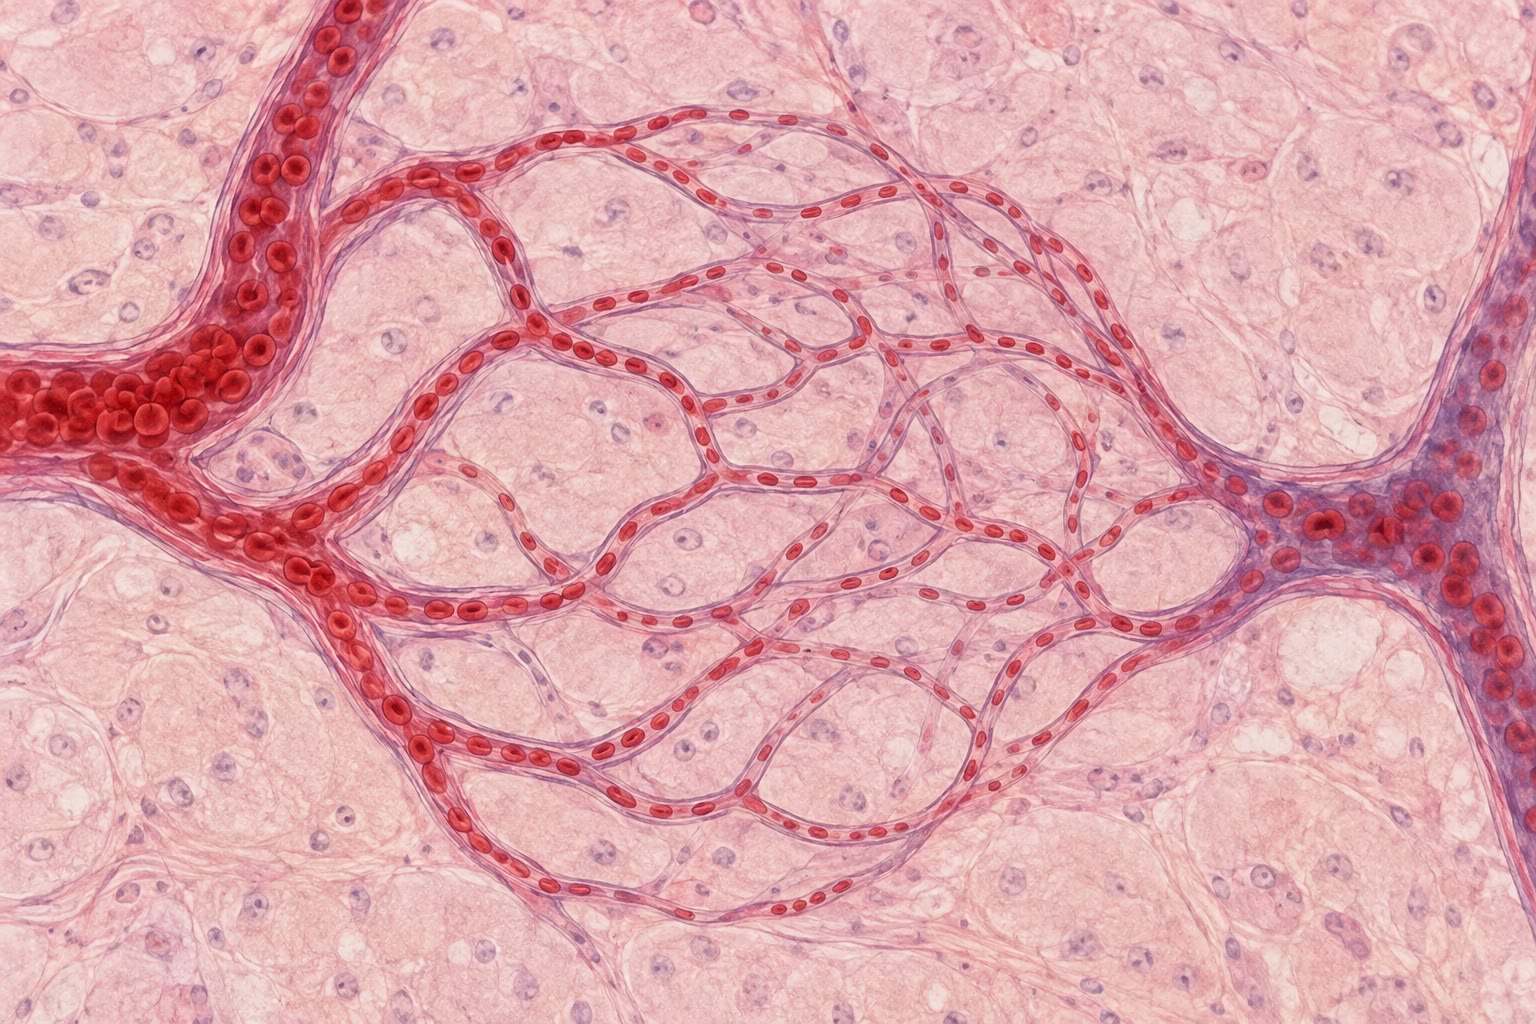
\includegraphics[width=0.55\linewidth]{images/book4/ai/b4-16-capillary-bed.jpg}

{\small Un lit \omterm{def:b2:blood-circulation:vessels}{capillaire}~: une \omterm{def:b2:blood-circulation:vessels}{artériole} alimente un réseau de
\omterm{def:b2:blood-circulation:vessels}{capillaires} où les \omterm{def:b2:blood-circulation:blood}{hématies} circulent en file indienne, puis se
rejoignent en une veinule.}
\end{omfigure}

\begin{theorem}[La loi de Poiseuille et la résistance vasculaire]\label{thm:b2:blood-circulation:poiseuille}
\index{loi de Poiseuille}\index{resistance vasculaire@résistance vasculaire}
Le débit stationnaire $Q$ d'un fluide de viscosité $\eta$ dans un tube
de rayon $r$ et de longueur $L$, sous une différence de pression
$\Delta P$, vaut
\[
Q = \frac{\pi r^{4}}{8\eta L}\,\Delta P, \qquad \text{d'où}\qquad
R \equiv \frac{\Delta P}{Q} = \frac{8\eta L}{\pi r^{4}} .
\]
La résistance diminue comme la \emph{puissance quatrième} du rayon~: une
\omterm{def:b2:blood-circulation:vessels}{artériole} qui réduit son rayon de \qty{20}{\%} multiplie sa résistance
par $1/0.8^{4} = 2.4$, et une \omterm{def:b2:blood-circulation:vessels}{artériole} qui le divise par deux, par 16.
C'est pourquoi quelques millimètres de muscle artériolaire peuvent
rediriger le \omterm{def:b2:blood-circulation:blood}{sang} du corps entier --- vers l'intestin après un repas,
vers les muscles pendant l'effort, vers la peau quand il fait chaud ---
et pourquoi la pression chute de \qty{95}{mmHg} dans les petites
\omterm{def:b2:blood-circulation:vessels}{artères} à \qty{35}{mmHg} à l'entrée des \omterm{def:b2:blood-circulation:vessels}{capillaires}, presque entièrement
à travers les \omterm{def:b2:blood-circulation:vessels}{artérioles}, tandis que la chute le long de l'aorte est
d'une fraction de millimètre de mercure.
\end{theorem}
\begin{proof}
En écoulement laminaire stationnaire, le fluide se déplace en couches
concentriques~; la force visqueuse entre les couches équilibre la
pression. Pour le cylindre de rayon $s < r$, la force de pression
$\pi s^{2}\Delta P$ est égale à la traînée visqueuse sur sa surface
$2\pi s L\,\eta\,(-\mathrm{d}v/
\mathrm{d}s)$, donc $\mathrm{d}v/\mathrm{d}s = -s\Delta P/(2\eta L)$
et, avec $v(r) = 0$, $v(s) = (\Delta P/4\eta L)(r^{2} - s^{2})$ --- un
profil parabolique. En intégrant la vitesse sur la section,
$Q = \int_{0}^{r} v\,2\pi s\,\mathrm{d}s = (\pi\Delta P/2\eta L)
\int_{0}^{r}(r^{2}s - s^{3})\,\mathrm{d}s = \pi r^{4}\Delta P/8\eta
L$. (Le \omterm{def:b2:blood-circulation:blood}{sang} n'est pas tout à fait un fluide simple et les \omterm{def:b2:blood-circulation:vessels}{artères} ne
sont pas rigides, mais la loi en puissance quatrième est assez valable
pour faire fonctionner un organisme.)
\end{proof}

\begin{theorem}[La continuité~: où le sang ralentit]\label{thm:b2:blood-circulation:continuity}
\index{equation de continuite@équation de continuité}
Le même volume par seconde traverse chaque niveau de l'arbre~: la
vitesse moyenne à un niveau vaut donc $v = Q/A$, où $A$ est la section
\emph{totale} de tous les vaisseaux de ce niveau. L'aorte
(\qty{3}{cm^2}) transporte \qty{5}{L/min} à \qty{28}{cm/s}~; les
\omterm{def:b2:blood-circulation:vessels}{capillaires}, d'une section totale voisine de \qty{3000}{cm^2}, le
transportent à \qty{0.03}{cm/s}, si bien qu'une \omterm{def:b2:blood-circulation:blood}{hématie} met environ trois
secondes à traverser un \omterm{def:b2:blood-circulation:vessels}{capillaire} --- assez de temps pour que son
dioxygène diffuse (\cref{ch:b2:unicellular-diversity}~: un micromètre
en une milliseconde). Les \omterm{def:b2:blood-circulation:vessels}{veines}, de section totale plus faible que les
\omterm{def:b2:blood-circulation:vessels}{capillaires}, accélèrent de nouveau le \omterm{def:b2:blood-circulation:blood}{sang} jusqu'à \qty{10}{cm/s} dans
les \omterm{def:b2:blood-circulation:vessels}{veines} caves. L'arbre est construit pour que le \omterm{def:b2:blood-circulation:blood}{sang} soit lent là
précisément où il doit échanger, et rapide partout ailleurs.
\end{theorem}
\begin{proof}
Conservation du volume~: ce qui entre dans un niveau par seconde en
ressort, si bien que $Q = A\,v$ est le même à chaque niveau.
$\qty{5}{L/min} =
\qty{83}{cm^3/s}$~; $83/3 = \qty{28}{cm/s}$~; $83/3000 =
\qty{0.028}{cm/s}$.
\end{proof}

\begin{omfigure}
\begin{tikzpicture}
\begin{axis}[
  width=0.9\linewidth, height=6.4cm,
  axis x line=bottom, axis y line=left,
  xmin=0, xmax=7, ymin=0, ymax=130,
  xtick={0.5,1.5,2.5,3.5,4.5,5.5,6.5},
  xticklabels={aorte, artères, artérioles, capillaires, veinules, veines, veines caves},
  x tick label style={font=\scriptsize, rotate=30, anchor=north east},
  ylabel={pression (\unit{mmHg})}, ylabel style={font=\small, omThm},
  tick label style={font=\small}, ytick={0,40,80,120},
  legend style={font=\scriptsize, at={(0.97,0.95)}, anchor=north east, draw=none},
  clip=false,
]
\addplot[very thick, omThm] coordinates {(0,120) (0.5,118) (1,110) (1.5,100) (2,95) (2.5,60) (3,35) (3.5,25) (4,15) (4.5,12) (5,8) (5.5,5) (6,4) (6.5,3) (7,2)};
\addlegendentry{pression moyenne}
\addplot[very thick, omThm, dashed] coordinates {(0,120) (0.5,120) (1,125) (1.5,120) (2,100)};
\addplot[very thick, omThm, dashed] coordinates {(0,80) (0.5,80) (1,80) (1.5,82) (2,88)};
\addlegendentry{systolique et diastolique}
\end{axis}
\begin{axis}[
  width=0.9\linewidth, height=6.4cm,
  axis x line=none, axis y line=right,
  xmin=0, xmax=7, ymin=0, ymax=32,
  ylabel={vitesse (\unit{cm/s})}, ylabel style={font=\small, omDef},
  tick label style={font=\small}, ytick={0,10,20,30},
  legend style={font=\scriptsize, at={(0.97,0.72)}, anchor=north east, draw=none},
  clip=false,
]
\addplot[very thick, omDef] coordinates {(0,28) (0.5,26) (1,18) (1.5,10) (2,5) (2.5,1.5) (3,0.3) (3.5,0.03) (4,0.3) (4.5,1.5) (5,4) (5.5,7) (6,9) (6.5,10) (7,10)};
\addlegendentry{vitesse moyenne}
\end{axis}
\end{tikzpicture}

{\small La pression (en rouge) et la vitesse moyenne (en bleu) le long de
la \omterm{def:b2:blood-circulation:circuits}{circulation systémique}. Les à-coups s'amortissent dans les \omterm{def:b2:blood-circulation:vessels}{artères},
la pression chute surtout à travers les \omterm{def:b2:blood-circulation:vessels}{artérioles}, et le \omterm{def:b2:blood-circulation:blood}{sang} est le
plus lent dans les \omterm{def:b2:blood-circulation:vessels}{capillaires}, dont la section totale est mille fois
celle de l'aorte.}
\end{omfigure}

\begin{theorem}[L'artère élastique comme réservoir]\label{thm:b2:blood-circulation:windkessel}
\index{Windkessel}\index{compliance!arterielle@artérielle}\index{pression differentielle@pression différentielle}
Le cœur éjecte par à-coups~; les tissus reçoivent un débit presque
régulier. Ce sont les grosses \omterm{def:b2:blood-circulation:vessels}{artères} qui lissent l'écoulement~: elles
se distendent pendant l'éjection, en stockant une partie du volume
d'éjection, et se rétractent pendant la diastole, en le propulsant plus
loin. Si les \omterm{def:b2:blood-circulation:vessels}{artères} ont une \emph{compliance} $C$ (volume stocké par
unité de pression) et les \omterm{def:b2:blood-circulation:vessels}{artérioles} une résistance $R$, alors, pendant
la diastole, la valve aortique étant fermée, la pression décroît selon
\[
P(t) = P_{s}\,e^{-t/RC},
\]
de sorte que la pression diastolique au bout d'une diastole de durée
$t_d$ vaut $P_s e^{-t_d/RC}$~: avec $R = \qty{1}{mmHg.s/mL}$, $C =
\qty{2}{mL/mmHg}$ et $t_d = \qty{0.8}{s}$, une pression systolique de
\qty{120}{mmHg} descend à \qty{80}{mmHg}. Une aorte plus rigide ($C$
plus faible, comme chez les personnes âgées) laisse la pression chuter
davantage entre deux battements et monter plus haut pendant
l'éjection~: la \emph{\omterm{thm:b2:blood-circulation:windkessel}{pression différentielle}} s'élargit, et le cœur
travaille contre un pic plus élevé.
\end{theorem}
\begin{proof}
Pendant la diastole, aucun \omterm{def:b2:blood-circulation:blood}{sang} n'entre dans les \omterm{def:b2:blood-circulation:vessels}{artères} et le \omterm{def:b2:blood-circulation:blood}{sang} en
sort par les \omterm{def:b2:blood-circulation:vessels}{artérioles} au débit $Q = P/R$~; le volume artériel diminue
selon
$\mathrm{d}V/\mathrm{d}t = -P/R$, et comme $\mathrm{d}V = C\,
\mathrm{d}P$, $C\,\mathrm{d}P/\mathrm{d}t = -P/R$, dont la solution est
l'exponentielle de constante de temps $RC$. Avec $RC = \qty{2}{s}$~:
$120\,e^{-0.4} = \qty{80}{mmHg}$.
\end{proof}

\section{Les échanges dans les capillaires}

\begin{proposition}[Deux types d'échanges]\label{prop:b2:blood-circulation:exchange}
\index{echanges capillaires@échanges capillaires}\index{forces de Starling}\index{oedeme@œdème}\index{lymphe}
À travers la paroi \omterm{def:b2:blood-circulation:vessels}{capillaire}, les solutés se déplacent par
\emph{diffusion} --- les gaz et les lipides à travers les cellules,
l'eau et les petits solutés par les fentes qui les séparent, sur une
surface énorme et une distance courte qui rendent le flux abondant (loi
de Fick, comme pour le \omterm{def:b2:mammal-reproduction:placenta}{placenta} du \cref{ch:b2:mammal-reproduction}) ---
et l'eau se déplace par \emph{écoulement en masse}, sous l'effet de
l'équilibre entre deux pressions. La pression hydrostatique dans le
\omterm{def:b2:blood-circulation:vessels}{capillaire}, $P_c$, pousse le liquide vers l'extérieur~; la \omterm{thm:b2:blood-circulation:oncotic}{pression
oncotique} des protéines plasmatiques, $\pi_c$, l'attire vers
l'intérieur (\emph{\omterm{prop:b2:blood-circulation:exchange}{forces de Starling}}). À l'extrémité artérielle,
$P_c \approx
\qty{35}{mmHg}$ dépasse $\pi_c \approx \qty{25}{mmHg}$ et le liquide
filtre vers l'extérieur~; à l'extrémité veineuse,
$P_c \approx \qty{15}{mmHg}$ et le liquide est réabsorbé~; sur l'ensemble du corps,
environ \qty{20}{L} filtrent chaque jour et \qty{17}{L} reviennent, et
le reliquat de \qty{3}{L}, avec les protéines qui ont fui, est recueilli
par les vaisseaux \emph{lymphatiques} et rendu aux \omterm{def:b2:blood-circulation:vessels}{veines} à la base du
cou. L'\emph{œdème} --- le gonflement dû au liquide dans les tissus ---
survient chaque fois que l'équilibre bascule~: pression veineuse élevée
(insuffisance cardiaque), protéines plasmatiques basses (dénutrition,
maladie du foie ou du rein), \omterm{def:b2:blood-circulation:vessels}{capillaires} perméables (inflammation) ou
lymphatiques obstrués.
\end{proposition}

\begin{omfigure}
\begin{tikzpicture}[every node/.style={font=\scriptsize}, >=stealth]
  % capillary
  \draw[thick, fill=omThm!10] (0,0) rectangle (9,1.2);
  \node[left] at (-0.1,0.6) {artériole};
  \node[right] at (9.1,0.6) {veinule};
  \draw[->, very thick, omThm] (0.3,0.6) -- (8.7,0.6);
  % pressures
  \node[above, align=center] at (1.5,1.3) {extrémité artérielle\\$P_c = 35$, $\pi_c = 25$};
  \node[above, align=center] at (7.5,1.3) {extrémité veineuse\\$P_c = 15$, $\pi_c = 25$};
  \foreach \x in {0.8,1.5,2.2} \draw[->, thick, omDef] (\x,0) -- (\x,-0.7);
  \node[below, align=center, omDef] at (1.5,-0.75) {bilan $+10$ mmHg~:\\filtration};
  \foreach \x in {6.8,7.5,8.2} \draw[->, thick, omDef] (\x,-0.7) -- (\x,0);
  \node[below, align=center, omDef] at (7.5,-0.75) {bilan $-10$ mmHg~:\\réabsorption};
  \draw[->, thick, omExo!70!black] (4.5,-0.4) -- (4.5,-1.6) node[below, align=center] {excédent vers la lymphe~:\\\qty{3}{L} par jour};
  \node[align=center] at (4.5,-0.15) {liquide interstitiel};
\end{tikzpicture}

{\small Les \omterm{prop:b2:blood-circulation:exchange}{forces de Starling} le long d'un \omterm{def:b2:blood-circulation:vessels}{capillaire}. La pression
hydrostatique pousse le liquide vers l'extérieur et la \omterm{thm:b2:blood-circulation:oncotic}{pression
oncotique} des protéines plasmatiques le rappelle~; la filtration à
l'extrémité artérielle dépasse la réabsorption à l'extrémité veineuse,
et la lymphe restitue la différence.}
\end{omfigure}

\begin{theorem}[La pression oncotique]\label{thm:b2:blood-circulation:oncotic}
\index{pression oncotique}\index{albumine}
Une solution contenant $c$ moles par litre d'un soluté incapable de
traverser une membrane exerce à travers celle-ci une pression osmotique
$\pi = cRT$ (van 't Hoff). L'albumine plasmatique, \qty{40}{g/L} d'une
protéine de masse molaire \qty{66}{kg/mol}, correspond à
$c = \qty{0.6}{mmol/L}$ et donne $\pi =
0.6\times 8.314\times 310 = \qty{1.55}{kPa} \approx \qty{12}{mmHg}$~;
les autres protéines et les ions supplémentaires que retient la charge
négative de l'albumine portent le total à environ \qty{25}{mmHg}. Le
chlorure de sodium du \omterm{def:b2:blood-circulation:blood}{plasma}, à \qty{150}{mmol/L}, exercerait
\qty{5800}{mmHg} --- mais il traverse librement la paroi \omterm{def:b2:blood-circulation:vessels}{capillaire} et
n'y exerce aucune pression. Ce qui compte pour le \omterm{def:b2:blood-circulation:vessels}{capillaire}, ce sont
les protéines~: divisez l'albumine par deux, comme dans une maladie
rénale qui la fait perdre dans l'urine, et l'attraction qui réabsorbe
diminue de moitié, le liquide s'accumule dans les tissus, et le patient
enfle.
\end{theorem}
\begin{proof}
$\qty{40}{g/L}/\qty{66000}{g/mol} = \qty{6.1e-4}{mol/L} =
\qty{0.61}{mol/m^3}$~; $\pi = cRT = 0.61\times 8.314\times 310 =
\qty{1570}{Pa}$~; $\qty{1}{mmHg} = \qty{133}{Pa}$, d'où \qty{11.8}{mmHg}.
La loi de van 't Hoff elle-même est la limite des solutions diluées
établie dans le volume de première année.
\end{proof}

\begin{example}[La circulation comme système de transport]\label{ex:b2:blood-circulation:transport}
Cinq litres par minute à travers \qty{600}{m^2} de paroi \omterm{def:b2:blood-circulation:vessels}{capillaire}~:
c'est un service de livraison sans égal. Il apporte à chaque cellule du
dioxygène à quelques diamètres cellulaires près (aucune cellule du corps
n'est à plus de \qty{20}{\micro m} d'un \omterm{def:b2:blood-circulation:vessels}{capillaire}), emporte son
$\mathrm{CO_2}$, son lactate et son urée, porte le glucose du foie au
cerveau et les acides gras des réserves adipeuses aux muscles, distribue
en une minute les hormones du \cref{ch:b2:cell-signalling} d'une glande
à tous les récepteurs du corps, transporte la chaleur du centre du corps
vers la peau et inversement, et achemine les leucocytes jusqu'à une
plaie en quelques heures. C'est aussi sa vulnérabilité~: un caillot, une
hémorragie ou une pompe défaillante arrêtent tout d'un coup, et le
cerveau, qui ne stocke aucun carburant, défaille en quelques secondes.
La suite de cette partie du livre traite de la pompe
(\cref{ch:b2:heart}) et de la régulation de la pression qui permet au
service de continuer lorsqu'on se lève, qu'on court ou qu'on saigne
(\cref{ch:b2:blood-pressure}).
\end{example}

\section{Exercices}

\begin{exercise}[$\star$]\label{exo:b2:blood-circulation:1}
Donner la composition du \omterm{def:b2:blood-circulation:blood}{sang} en volume, ainsi que le nombre, la taille
et la fonction de chaque composant cellulaire.
\end{exercise}

\begin{exercise}[$\star$]\label{exo:b2:blood-circulation:2}
Schématiser la circulation d'un poisson et celle d'un mammifère,
indiquer les pressions, et dire ce qu'apporte la circulation double.
\end{exercise}

\begin{exercise}[$\star$]\label{exo:b2:blood-circulation:3}
Pour chaque type de vaisseau --- \omterm{def:b2:blood-circulation:vessels}{artère}, \omterm{def:b2:blood-circulation:vessels}{artériole}, \omterm{def:b2:blood-circulation:vessels}{capillaire}, \omterm{def:b2:blood-circulation:vessels}{veine}
--- donner la structure de la paroi et la fonction qu'elle sert.
\end{exercise}

\begin{exercise}[$\star$]\label{exo:b2:blood-circulation:4}
Reconstituer l'argument quantitatif de Harvey avec des valeurs
actuelles~: \qty{70}{mL} par battement, \num{72} battements par minute,
\qty{5}{L} de \omterm{def:b2:blood-circulation:blood}{sang}.
\end{exercise}

\begin{exercise}[$\star\star$]\label{exo:b2:blood-circulation:5}
Calculer par la \omterm{thm:b2:blood-circulation:poiseuille}{loi de Poiseuille} la chute de pression le long de
l'aorte (rayon \qty{1.25}{cm}, longueur \qty{40}{cm},
$\eta = \qty{3e-3}{Pa.s}$) transportant \qty{5}{L/min}, en pascals et
en mmHg. Commenter.
\end{exercise}

\begin{exercise}[$\star\star$]\label{exo:b2:blood-circulation:6}
Une \omterm{def:b2:blood-circulation:vessels}{artériole} de rayon \qty{15}{\micro m} se contracte jusqu'à
\qty{12}{\micro m}, puis se dilate jusqu'à \qty{20}{\micro m}. De quel
facteur sa résistance change-t-elle dans chaque cas, et son débit à
pression constante~?
\end{exercise}

\begin{exercise}[$\star\star$]\label{exo:b2:blood-circulation:7}
L'aorte a une section de \qty{3}{cm^2} et les \omterm{def:b2:blood-circulation:vessels}{capillaires} une section
totale de \qty{3000}{cm^2}~; le débit est de \qty{5}{L/min}. Calculer la
vitesse moyenne dans chacun, et le temps qu'une \omterm{def:b2:blood-circulation:blood}{hématie} passe dans un
\omterm{def:b2:blood-circulation:vessels}{capillaire} de \qty{1}{mm}. Pendant l'effort, le débit monte à
\qty{25}{L/min} et les \omterm{def:b2:blood-circulation:vessels}{capillaires} musculaires s'ouvrent~: qu'advient-il
du temps de transit~?
\end{exercise}

\begin{exercise}[$\star\star$]\label{exo:b2:blood-circulation:8}
Avec $P_c = 35$ et \qty{15}{mmHg} aux deux extrémités, $\pi_c =
\qty{25}{mmHg}$ et des pressions interstitielles négligeables, calculer
la pression nette de filtration à chaque extrémité. Que se passe-t-il si
la pression veineuse augmente de sorte que $P_c$ à l'extrémité veineuse
vaut \qty{28}{mmHg}~?
\end{exercise}

\begin{exercise}[$\star\star$]\label{exo:b2:blood-circulation:9}
Calculer la \omterm{thm:b2:blood-circulation:oncotic}{pression oncotique} de \qty{40}{g/L} d'albumine
(\qty{66}{kg/mol}) à \qty{37}{\celsius}, et celle de \qty{20}{g/L}.
Pourquoi le sodium du \omterm{def:b2:blood-circulation:blood}{plasma}, à \qty{150}{mmol/L}, ne contribue-t-il en
rien à l'équilibre de Starling~?
\end{exercise}

\begin{exercise}[$\star\star\star$]\label{exo:b2:blood-circulation:10}
Avec $R = \qty{1}{mmHg.s/mL}$ et $C = \qty{2}{mL/mmHg}$, calculer la
pression diastolique au bout de \qty{0.8}{s} à partir d'une pression
systolique de \qty{120}{mmHg}. Refaire le calcul pour une aorte deux
fois moins compliante. Expliquer pourquoi la \omterm{thm:b2:blood-circulation:windkessel}{pression différentielle} des
personnes âgées est élevée, et ce qu'elle coûte au cœur.
\end{exercise}

\begin{exercise}[$\star\star\star$]\label{exo:b2:blood-circulation:11}
La résistance systémique vaut $R = (P_{\text{art}} - P_{\text{ven}})/Q$.
La calculer au repos ($95 - 5$ mmHg, \qty{5}{L/min}) et à l'effort
($110 - 5$, \qty{25}{L/min}). De quel facteur le rayon artériolaire moyen
doit-il avoir changé, si les \omterm{def:b2:blood-circulation:vessels}{artérioles} portent toute la résistance~?
\end{exercise}

\begin{exercise}[$\star\star\star$]\label{exo:b2:blood-circulation:12}
«~La circulation est construite pour que le \omterm{def:b2:blood-circulation:blood}{sang} soit lent là où il doit
échanger et rapide partout ailleurs.~» Discuter à l'aide de l'\omterm{thm:b2:blood-circulation:continuity}{équation
de continuité}, de la \omterm{thm:b2:blood-circulation:poiseuille}{loi de Poiseuille} et de la géométrie de l'arbre, et
dire pourquoi une \omterm{def:b2:blood-circulation:circuits}{circulation ouverte} ne peut pas faire de même.
\end{exercise}

\section{Problème~: la circulation en chiffres}

\begin{problem}[{Problème du week-end --- le calcul de Harvey refait, les
pressions et les vitesses de l'arbre vasculaire calculées par les lois
de Poiseuille et de continuité, la filtration capillaire journalière mise
en équilibre et le lissage par l'aorte modélisé, jusqu'au débit
cardiaque, à la chute de pression artériolaire, au filtrat de la journée
et à la pression diastolique}]
\label{pb:b2:blood-circulation:1}
Données~: volume d'éjection \qty{70}{mL}, fréquence cardiaque
\qty{72}{min^{-1}}, volume sanguin \qty{5}{L}, $\eta = \qty{3e-3}{Pa.s}$,
$\qty{1}{mmHg} =
\qty{133}{Pa}$. Aorte~: rayon \qty{1.25}{cm}, longueur \qty{40}{cm}.
\omterm{def:b2:blood-circulation:vessels}{Artérioles}~: $3\times 10^{6}$ en parallèle, chacune de rayon
\qty{15}{\micro m} et de longueur \qty{1}{mm}. \omterm{def:b2:blood-circulation:vessels}{Capillaires}~: $4\times
10^{10}$, de rayon \qty{3}{\micro m} et de longueur \qty{1}{mm}, dont un
quart ouverts au repos. Starling~: $P_c$ de 35 à \qty{15}{mmHg} le long
d'un \omterm{def:b2:blood-circulation:vessels}{capillaire}, $\pi_c = \qty{25}{mmHg}$. Windkessel~: $C =
\qty{2}{mL/mmHg}$, diastole de \qty{0.8}{s}.

\medskip
\noindent\textbf{Partie I --- Le calcul de Harvey.}
\begin{enumerate}
  \item Calculer le débit cardiaque en litres par minute et par jour.
  \item Combien de fois le volume sanguin circule-t-il en une journée~?
  \item Harvey estimait à 2~onces (\qty{57}{g}) le contenu du cœur à
        chaque battement, dont il supposait au moins un quart expulsé,
        à 72 battements par minute. Quelle masse de \omterm{def:b2:blood-circulation:blood}{sang} cela
        donnait-il par heure, et comment se comparait-elle au poids
        d'un homme~?
  \item Pourquoi était-ce un argument en faveur d'une circulation
        plutôt que d'une production et d'une consommation continues~?
  \item Décrire l'expérience de la ligature et ce que montraient les
        valvules.
  \item Que Harvey ne pouvait-il pas voir, et qui l'a vu~?
\end{enumerate}

\medskip
\noindent\textbf{Partie II --- L'arbre.}
\begin{enumerate}[resume]
  \item Calculer la vitesse moyenne dans l'aorte.
  \item Calculer par la \omterm{thm:b2:blood-circulation:poiseuille}{loi de Poiseuille} la chute de pression le long
        de l'aorte, en mmHg.
  \item Calculer la résistance d'une \omterm{def:b2:blood-circulation:vessels}{artériole} et celle des $3\times
        10^{6}$ \omterm{def:b2:blood-circulation:vessels}{artérioles} en parallèle.
  \item Calculer la chute de pression à travers les \omterm{def:b2:blood-circulation:vessels}{artérioles} au débit
        de repos, en mmHg.
  \item Calculer la section totale des \omterm{def:b2:blood-circulation:vessels}{capillaires} ouverts et la vitesse
        moyenne dans ces \omterm{def:b2:blood-circulation:vessels}{capillaires}~; puis le temps de transit dans l'un
        d'eux.
  \item Les \omterm{def:b2:blood-circulation:vessels}{artérioles} se contractent de sorte que leur rayon diminue de
        \qty{10}{\%}. Recalculer la chute de pression. Que doit faire le
        cœur pour maintenir le même débit~?
\end{enumerate}

\medskip
\noindent\textbf{Partie III --- Les \omterm{def:b2:blood-circulation:vessels}{capillaires}.}
\begin{enumerate}[resume]
  \item Calculer la pression nette de filtration à l'extrémité
        artérielle, à l'extrémité veineuse et au milieu (en supposant que
        $P_c$ décroît linéairement).
  \item Diviser le \omterm{def:b2:blood-circulation:vessels}{capillaire} en une moitié qui filtre et une moitié qui
        réabsorbe, et estimer le liquide filtré et réabsorbé par jour
        dans l'ensemble du corps, en prenant pour pressions nettes
        moyennes sur chaque moitié $+10$ et
        \qty{-8.5}{mmHg}, et en supposant que chaque moitié déplace
        \qty{2}{L} par jour et par mmHg.
  \item En déduire le débit de lymphe.
  \item L'albumine plasmatique tombe à \qty{20}{g/L}. Recalculer $\pi_c$
        (en supposant qu'elle est proportionnelle à l'albumine) et les
        pressions nettes aux deux extrémités. Que se passe-t-il~?
  \item La pression veineuse augmente de sorte que $P_c$ va de 35 à
        \qty{28}{mmHg}. Recalculer la pression nette moyenne et le bilan
        journalier. Où va le liquide~?
  \item Calculer la surface \omterm{def:b2:blood-circulation:vessels}{capillaire} totale (des cylindres, tous les
        \omterm{def:b2:blood-circulation:vessels}{capillaires}) et le temps que met une molécule à diffuser jusqu'à
        une cellule située à \qty{20}{\micro m} d'un \omterm{def:b2:blood-circulation:vessels}{capillaire}
        ($D = \qty{1e-9}{m^2/s}$).
\end{enumerate}

\medskip
\noindent\textbf{Partie IV --- L'aorte comme réservoir.}
\begin{enumerate}[resume]
  \item Calculer la résistance systémique à partir d'une pression moyenne
        de \qty{93}{mmHg}, d'une pression veineuse de \qty{3}{mmHg} et du
        débit de repos, en \unit{mmHg.s/mL}.
  \item Calculer la constante de temps $RC$ et la pression diastolique au
        bout de \qty{0.8}{s} à partir d'une pression systolique de
        \qty{120}{mmHg}.
  \item Refaire le calcul pour $C = \qty{1}{mL/mmHg}$. Qu'est devenue la
        \omterm{thm:b2:blood-circulation:windkessel}{pression différentielle}~?
  \item La fréquence cardiaque monte à \num{120} et la diastole se réduit
        à \qty{0.3}{s}. Calculer la pression diastolique.
  \item Sur les \qty{70}{mL} éjectés, quelle quantité est stockée dans
        les \omterm{def:b2:blood-circulation:vessels}{artères} pendant la systole si la pression augmente de
        \qty{20}{mmHg}~? Où va le reste~?
  \item Expliquer pourquoi les \omterm{def:b2:blood-circulation:vessels}{artères} coronaires, qui se remplissent en
        diastole, dépendent de la rétraction de l'aorte.
  \item Énoncer le résultat~: le débit cardiaque, la chute de pression
        artériolaire, le filtrat net de la journée, et la pression
        diastolique pour $C = 2$ et $C = 1$.
\end{enumerate}
\end{problem}
